\section{Resultados}\label{sec:resultados}
A continuación, se presentan los casos de estudio que se han realizado para diferentes simulaciones del juego
de la vida en dos y tres dimensiones, y sus respectivos resultados.
Para cada caso, se detallan los parámetros de entrada fijos utilizados, seguido de una o más figuras en el que
se muestra la evolución del sistema en cada paso temporal en valores extremos, y finalmente, un análisis del
observable en función de la densidad de celdas vivas en el dominio inicial.

\subsection{Conway en 2D}\label{subsec:conway-en-2d}

Como primer modelo, se ha estudiado el reconocido juego de la vida de Conway en dos dimensiones.
Para ello, se fija los siguientes parámetros de entrada:

\begin{itemize}
    \item $border = (0, 0) \times (100, 100)$
    \item $condition = MOORE$
    \item $r = 1$
    \item $shouldKeepAlive = [2, 3]$
    \item $shouldRevive = [3]$
    \item $initialDomainProportion = 0.16$
\end{itemize}

Variando el parámetro $initialLiveCellsProportion$ entre 0.1 y 0.9, se ha analizado la cantidad de celdas vivas
a lo largo de los pasos temporales.

\begin{figure}[H]
    \centering
    \includegraphics[width=0.8\linewidth]{conway2d/size_i10}
    \caption{Cantidad de celdas vivas en el tiempo del sistema de Conway con $initialLiveCellsProportion = 0.1$}
    \label{fig:conway2d_i10}
\end{figure}
\begin{figure}[H]
    \centering
    \includegraphics[width=0.8\linewidth]{conway2d/size_i90}
    \caption{Cantidad de celdas vivas en el tiempo del sistema de Conway con $initialLiveCellsProportion = 0.9$}
    \label{fig:conway2d_i90}
\end{figure}

Como se puede apreciar en las figs. \ref{fig:conway2d_i10} y \ref{fig:conway2d_i90}, el sistema alcanza el equilibrio
antes del paso temporal 900, por lo que se hace el análisis del observable en el paso temporal mencionado.
En base a las figuras anteriores, se ha observado la cantidad de celdas vivas en función de la densidad de celdas
vivas en el dominio inicial.

\begin{figure}[H]
    \centering
    \includegraphics[width=0.8\linewidth]{conway2d/size_vs_input}
    \caption{Cantidad de celdas vivas en función del input para el sistema de Conway 2D}
    \label{fig:conway2d_size_vs_input}
\end{figure}

A partir de la fig. \ref{fig:conway2d_size_vs_input}, se puede analizar que a medida que aumenta la densidad inicial de
celdas vivas, aunque con algunas oscilaciones, la cantidad de celdas vivas en el equilibrio también.
También se ha estudiado la pendiente de crecimiento de la cantidad de celdas vivas en función del input.
Este se calcula como la variación de la cantidad de celdas vivas entre el paso temporal inicial y el paso temporal
de equilibrio dividido por la cantidad de pasos temporales; es decir, si $m_{s}$ es la pendiente, $n_{0}$ es la
cantidad de celdas vivas en el paso temporal inicial y $n_{eq}$ es la cantidad de celdas vivas en el equilibrio,
entonces $m_{s} = \frac{n_{eq} - n_0}{t_{eq} - t_{0}}$.

\begin{figure}[H]
    \centering
    \includegraphics[width=0.8\linewidth]{conway2d/size_slope_vs_input}
    \caption{Pendiente de crecimiento de cantidad de celdas vivas en función del input para el sistema de Conway 2D}
    \label{fig:conway2d_size_slope_vs_input}
\end{figure}

Se puede comprobar en la fig. \ref{fig:conway2d_size_slope_vs_input} que la pendiente de crecimiento es negativa
para cualquier valor de $initialLiveCellsProportion$, y su tendencia es más pronunciada a medida que aumenta la
densidad inicial de celdas vivas.

Por otro lado, se ha estudiado la distancia de la celda viva más lejana al centro de la matriz en función del
paso temporal.

\begin{figure}[H]
    \centering
    \includegraphics[width=0.8\linewidth]{conway2d/distance_i10}
    \caption{Distancia de la celda viva más lejana al centro en función del tiempo con $initialLiveCellsProportion = 0.1$}
    \label{fig:conway2d_d10}
\end{figure}
\begin{figure}[H]
    \centering
    \includegraphics[width=0.8\linewidth]{conway2d/distance_i90}
    \caption{Distancia de la celda viva más lejana al centro en función del tiempo con $initialLiveCellsProportion = 0.9$}
    \label{fig:conway2d_d90}
\end{figure}

Con estos resultados, dado que, en la mayoría de los casos, la simulación finaliza porque una celda viva llega al borde de la matriz,
se ha analizado el tiempo de finalización y la rapidez con la que se aleja la celda viva más lejana al centro, en función de la densidad de celdas vivas en el dominio inicial.
Con respecto al último observable, se ha calculado la pendiente de la distancia de la celda viva más lejana al centro en función del paso temporal;
es decir, si $m_{d}$ es la pendiente, $d_{0}$ es la distancia de la celda viva más lejana al centro en el paso temporal inicial y $d_{eq}$ en el equilibrio, entonces $m_{d} = \frac{d_{eq} - d_0}{t_{eq} - t_{0}}$.

\begin{figure}[H]
    \centering
    \includegraphics[width=0.8\linewidth]{conway2d/time_vs_input}
    \caption{Tiempo de finalización en función del input para el sistema de Conway 2D}
    \label{fig:conway2d_time_vs_input}
\end{figure}
\begin{figure}[H]
    \centering
    \includegraphics[width=0.8\linewidth]{conway2d/distance_slope_vs_input}
    \caption{Pendiente de alejamiento de la celda viva más lejana al centro en función del input para el sistema de Conway 2D}
    \label{fig:conway2d_distance_slope_vs_input}
\end{figure}

Se puede observar en ambas figs. \ref{fig:conway2d_time_vs_input} y \ref{fig:conway2d_distance_slope_vs_input} que cuando
$initialLiveCellsProportion = 0.6$ se obtiene el menor tiempo de finalización y la mayor rapidez de alejamiento de la celda viva más lejana al centro.

\subsection{Cuarentena en 2D}\label{subsec:cuarentena-2D}

El objetivo de este sistema es limitar el crecimiento en cantidad de celdas vivas a únicamente la sección inicial o una subparte de esta. Para ello
se utilizaron los siguientes parámetros:

\begin{itemize}
    \item $border = (0, 0) \times (100, 100)$
    \item $condition = MOORE$
    \item $r = 1$
    \item $shouldKeepAlive = [1, 2, 3, 4, 5, 6, 7, 8]$
    \item $shouldRevive = [4, 5, 6, 7, 8]$
    \item $initialDomainProportion = 0.16$
\end{itemize}

2.4.1 Para cada input o parámetro a estudiar, primero mostrar una animación característica del 
sistema (pueden ser dos, con dos valores extremos del input para ver ejemplos de distintos 
comportamientos). La idea de esto es ilustrar la dinámica del sistema para situar el contexto de los 
resultados a mostrar. Acuerdense de poner un fotograma representativo y después el link a youtube 

A continuación se puede observar una animación característica del sistema con un input de 0.5:

\begin{figure}[H]
    \centering
    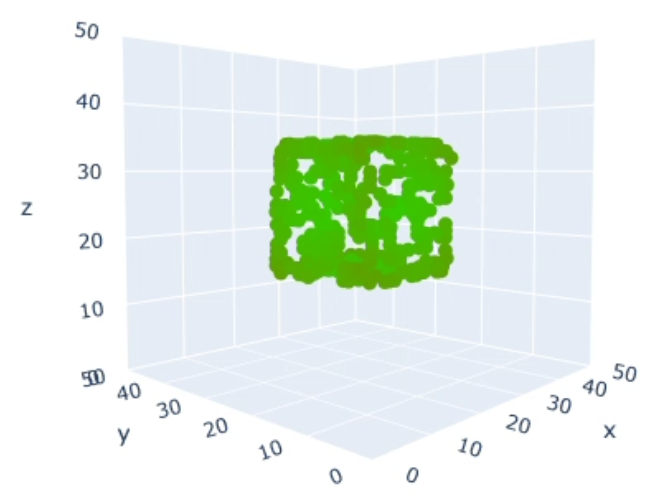
\includegraphics[width=0.8\linewidth]{cuarentena2d/thumbnail_i50}
    \caption{Fotograma de la animación de Cuarentena con $initialLiveCellsProportion = 0.5$}
    \label{fig:thumbnailcuarentena2d_i50}
\end{figure}

Enlace a la animación completa: https://youtu.be/hAECaws6P90

2.4.2 Luego mostrar una figura del observable o métrica (que se calcula a partir de los outputs 
directos de la simulación) en función del tiempo. Explicar entonces cual será el escalar que 
caracteriza ese proceso (por ejemplo el promedio de la evolución temporal en el estado 
estacionario, la tasa de crecimiento, etc.). Solo mostrar evoluciones típicas, de valores extremos 
del rango de parámetros, para validar las definiciones de los observables. Las evoluciones en sí 
no son los resultados definitivos, por lo tanto no deben ser extenso lo que se muestre de las 
mismas solo para justificar el observable (escalar) que se calculará a partir de estas.

A diferencia de los otros sistemas, en este no solo se varió el parámetro $initialLiveCellsProportion$ entre 0.1 y 0.9 con un paso de 0.1, 
sino que además se agregaron corridas con el parámetro valiendo 0.05 y 0.15.

A continuación podemos observar cómo evoluciona la cantidad de celdas vidas en función del tiempo para disitntos valores del parámetro $initialLiveCellsProportion$

\begin{figure}[H]
    \centering
    \includegraphics[width=0.8\linewidth]{cuarentena2d/size_i10}
    \caption{Cantidad de celdas vivas en el tiempo del sistema de Cuarentena con $initialLiveCellsProportion = 0.1$}
    \label{fig:cuarentena2d_i10}
\end{figure}
\begin{figure}[H]
    \centering
    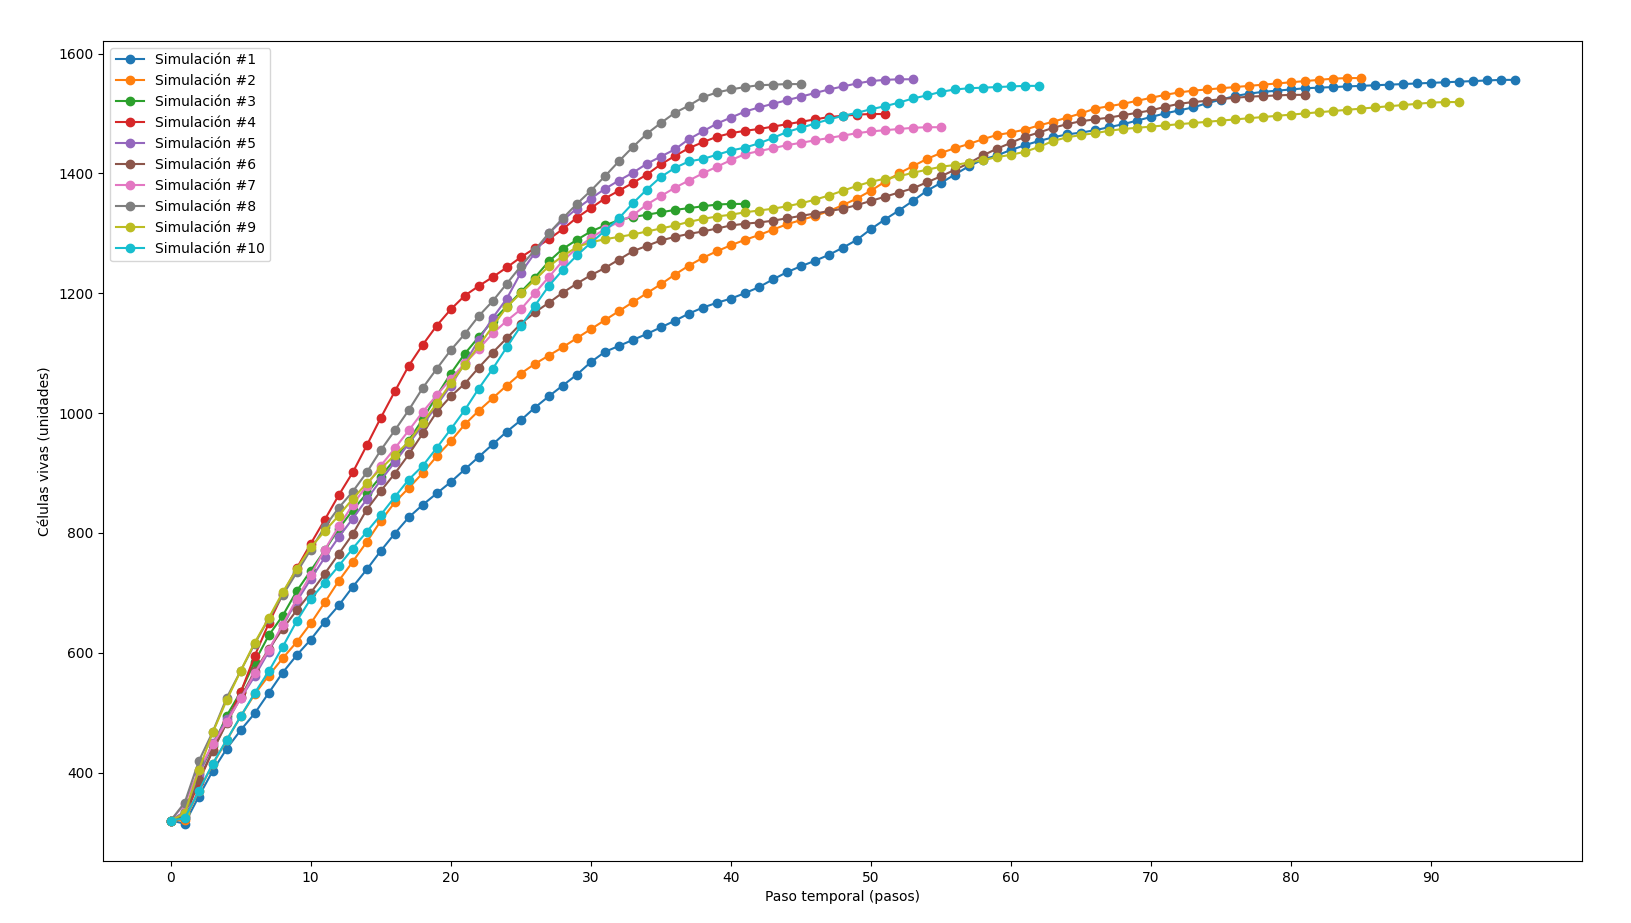
\includegraphics[width=0.8\linewidth]{cuarentena2d/size_i20}
    \caption{Cantidad de celdas vivas en el tiempo del sistema de Cuarentena con $initialLiveCellsProportion = 0.2$}
    \label{fig:cuarentena2d_i20}
\end{figure}
\begin{figure}[H]
    \centering
    \includegraphics[width=0.8\linewidth]{cuarentena2d/size_i80}
    \caption{Cantidad de celdas vivas en el tiempo del sistema de Cuarentena con $initialLiveCellsProportion = 0.8$}
    \label{fig:cuarentena2d_i80}
\end{figure}

La distancia de la celda viva más lejana al centro en función del tiempo es prácticamente idéntica para todos los inputs utilizados.

Lo interesante de este sistema no es la cantidad de celdas vivas en el momento de equilibrio debido a que si utilizamos $initialLiveCellsProportion$
por lo que hacemos hincapie en el crecimiento de cantidad de células vivas.

SUPONGO QUE HAY QUE HABLAR ACERCA DE CÓMO SE HIZO EL CÁLCULO DE CRECIMIENTO 


2.4.3 Después presentar la figura del input vs. observable, con promedio y barras de error o tablas 
con promedio y error. 

A continuación observamos el análisis del observable

\begin{figure}[H]
    \centering
    \includegraphics[width=0.8\linewidth]{cuarentena2d/observable}
    \caption{Pendiente de crecimiento de cantidad de celdas vivas en función del input para el sistema Cuarentena 2D}
    \label{fig:cuarentena2d_observable}
\end{figure}







\subsection{Expansión Circular en 2D}\label{subsec:expansion-circular-2D}

El objetivo de este sistema es obtener un crecimiento similar en todas las direcciones. Para ello se utilizaron los siguientes parámetros:

\begin{itemize}
    \item $border = (0, 0) \times (100, 100)$
    \item $condition = MOORE$
    \item $r = 1$
    \item $shouldKeepAlive = [0, 1, 4, 5, 6, 7, 8]$
    \item $shouldRevive = [2, 3]$
    \item $initialDomainProportion = 0.16$
\end{itemize}

2.4.1 Para cada input o parámetro a estudiar, primero mostrar una animación característica del 
sistema (pueden ser dos, con dos valores extremos del input para ver ejemplos de distintos 
comportamientos). La idea de esto es ilustrar la dinámica del sistema para situar el contexto de los 
resultados a mostrar. Acuerdense de poner un fotograma representativo y después el link a youtube 

A continuación se puede observar una animación característica del sistema con un input de 0.6:

\begin{figure}[H]
    \centering
    \includegraphics[width=0.8\linewidth]{circular2d/thumbnail}
    \caption{Fotograma de la animación de Expansión Circular con $initialLiveCellsProportion = 0.6$}
    \label{fig:thumbnailcircular2d_i60}
\end{figure}

Enlace a la animación completa: https://youtu.be/AIikxHN6VO4

2.4.2 Luego mostrar una figura del observable o métrica (que se calcula a partir de los outputs 
directos de la simulación) en función del tiempo. Explicar entonces cual será el escalar que 
caracteriza ese proceso (por ejemplo el promedio de la evolución temporal en el estado 
estacionario, la tasa de crecimiento, etc.). Solo mostrar evoluciones típicas, de valores extremos 
del rango de parámetros, para validar las definiciones de los observables. Las evoluciones en sí 
no son los resultados definitivos, por lo tanto no deben ser extenso lo que se muestre de las 
mismas solo para justificar el observable (escalar) que se calculará a partir de estas.


Variando el parámetro $initialLiveCellsProportion$ entre 0.1 y 0.9 con un step de 0.1, se ha analizado la cantidad de celdas vivas en función
del tiempo.

\begin{figure}[H]
    \centering
    \includegraphics[width=0.8\linewidth]{circular2d/size_i10}
    \caption{Cantidad de celdas vivas en el tiempo del sistema de Expansión Circular con $initialLiveCellsProportion = 0.1$}
    \label{fig:circular2d_i10}
\end{figure}
\begin{figure}[H]
    \centering
    \includegraphics[width=0.8\linewidth]{circular2d/size_i80}
    \caption{Cantidad de celdas vivas en el tiempo del sistema de Expansión Circular con $initialLiveCellsProportion = 0.8$}
    \label{fig:circular2d_i80}
\end{figure}


Es posible visualizar que con ambos parámetros la simulación termina después de 33 pasos, esto se debe a que con este sistema, la simulación
siempre termina por haber llegado al borde. Por lo cual no es de interés analizar la distancia al centro de la celda viva más lejana, ya que
crece de manera lineal sin importar el valor de $initialLiveCellsProportion$.

Por otro lado, sí es interesante utilizar como observable la cantidad de celdas vivas en el instante final de la simulación, a continuación se
grafica este mismo en función del valor de $initialLiveCellsProportion$

2.4.3 Después presentar la figura del input vs. observable, con promedio y barras de error o tablas 
con promedio y error. 


\begin{figure}[H]
    \centering
    \includegraphics[width=0.8\linewidth]{circular2d/observable}
    \caption{Cantidad de celdas vivas en función del input para el sistema Expansión Circular}
    \label{fig:circular2d_observable}
\end{figure}






\subsection{Expansión Cúbica}\label{subsec:cubito-3D}

El objetivo de este sistema es crecer en cada paso 1 posición más alejada del centro, pero sin que la cantidad de celdas vivas crezca en todos los pasos.

\begin{itemize}
    \item $border = (0, 0) \times (100, 100)$
    \item $condition = MOORE$
    \item $r = 1$
    \item $shouldKeepAlive = [1, 2, 3, 4, 5, 6, 7, 8]$
    \item $shouldRevive = [4, 5, 6, 7, 8]$
    \item $initialDomainProportion = 0.16$
\end{itemize}


A continuación se puede observar una animación característica del sistema con un input de 0.9:

\begin{figure}[H]
    \centering
    \includegraphics[width=0.8\linewidth]{cubo3d/thumbnail}
    \caption{Fotograma de la animación de Expansión Cúbica con $initialLiveCellsProportion = 0.9$}
    \label{fig:thumbnailcubo3d_i90}
\end{figure}

Enlace a la animación completa: https://youtu.be/Zu9bqnto0ak


2.4.2 Luego mostrar una figura del observable o métrica (que se calcula a partir de los outputs 
directos de la simulación) en función del tiempo. Explicar entonces cual será el escalar que 
caracteriza ese proceso (por ejemplo el promedio de la evolución temporal en el estado 
estacionario, la tasa de crecimiento, etc.). Solo mostrar evoluciones típicas, de valores extremos 
del rango de parámetros, para validar las definiciones de los observables. Las evoluciones en sí 
no son los resultados definitivos, por lo tanto no deben ser extenso lo que se muestre de las 
mismas solo para justificar el observable (escalar) que se calculará a partir de estas.


Variando el parámetro $initialLiveCellsProportion$ entre 0.1 y 0.9 con un step de 0.1, se ha analizado la cantidad de celdas vivas en función
del tiempo.

\begin{figure}[H]
    \centering
    \includegraphics[width=0.8\linewidth]{cubo3d/size_i10}
    \caption{Cantidad de celdas vivas en el tiempo del sistema de Expansión Cúbica con $initialLiveCellsProportion = 0.1$}
    \label{fig:cubo3d_i10}
\end{figure}
\begin{figure}[H]
    \centering
    \includegraphics[width=0.8\linewidth]{cubo3d/size_i80}
    \caption{Cantidad de celdas vivas en el tiempo del sistema de Expansión Cúbica con $initialLiveCellsProportion = 0.8$}
    \label{fig:cubo3d_i80}
\end{figure}


Es posible visualizar que con ambos parámetros la simulación termina después de 19 pasos, esto se debe a que con este sistema, la simulación
siempre termina por haber llegado al borde. Por lo cual no es de interés analizar la distancia al centro de la celda viva más lejana, ya que
crece de manera lineal sin importar el valor de $initialLiveCellsProportion$.

Debido a la naturaleza del crecimiento resulta interesante analizar la pendiente de crecimiento en función del input.

2.4.3 Después presentar la figura del input vs. observable, con promedio y barras de error o tablas 
con promedio y error. 


\begin{figure}[H]
    \centering
    \includegraphics[width=0.8\linewidth]{cubo3d/observable}
    \caption{Pendiente de crecimiento de cantidad de celdas vivas en función del input para el sistema Expansión Circular}
    \label{fig:cubo3d_observable}
\end{figure}


\subsection{Conway en 3D}\label{subsec:conway-en-3d}

Luego de analizar el sistema de Conway en dos dimensiones en la sección \ref{subsec:conway-en-2d},
se ha decidido estudiar el mismo sistema en tres dimensiones, con el fin de comprobar si los resultados
que se han obtenido en el caso bidimensional se mantienen en el caso tridimensional.
Para ello, se fijan los siguientes parámetros de entrada:
\begin{itemize}
    \item $border = (0, 0, 0) \times (50, 50, 50)$
    \item $condition = MOORE$
    \item $r = 1$
    \item $shouldKeepAlive = [2, 3]$
    \item $shouldRevive = [3]$
    \item $initialDomainProportion = 0.064$
\end{itemize}

Variando el parámetro $initialLiveCellsProportion$ entre 0.1 y 0.9, se ha analizado la cantidad de celdas vivas
a lo largo de los pasos temporales.

\begin{figure}[H]
    \centering
    \includegraphics[width=0.8\linewidth]{conway3d/size_i10}
    \caption{Cantidad de celdas vivas en el tiempo del sistema de Conway 3D con $initialLiveCellsProportion = 0.1$}
    \label{fig:conway3d_i10}
\end{figure}
\begin{figure}[H]
    \centering
    \includegraphics[width=0.8\linewidth]{conway3d/size_i90}
    \caption{Cantidad de celdas vivas en el tiempo del sistema de Conway 3D con $initialLiveCellsProportion = 0.9$}
    \label{fig:conway3d_i90}
\end{figure}

Como se puede apreciar en las figs. \ref{fig:conway3d_i10} y \ref{fig:conway3d_i90}, el sistema alcanza el equilibrio
antes del paso temporal 30, por lo que se hace el análisis del observable en el paso temporal mencionado.
En base a las figuras anteriores, se ha observado la cantidad de celdas vivas en función de la densidad de celdas
vivas en el dominio inicial.

\begin{figure}[H]
    \centering
    \includegraphics[width=0.8\linewidth]{conway3d/size_vs_input}
    \caption{Cantidad de celdas vivas en función del input para el sistema de Conway 3D}
    \label{fig:conway3d_size_vs_input}
\end{figure}

A partir de la fig. \ref{fig:conway3d_size_vs_input}, se puede analizar que la cantidad
de celdas vivas en el equilibrio alcanza un máximo cuando $initialLiveCellsProportion = 0.5$, y luego
disminuye a medida que aumenta la densidad inicial de celdas vivas.
También se ha estudiado la pendiente de crecimiento de la cantidad de celdas vivas en función del input.

\begin{figure}[H]
    \centering
    \includegraphics[width=0.8\linewidth]{conway3d/size_slope_vs_input}
    \caption{Pendiente de crecimiento de cantidad de celdas vivas en función del input para el sistema de Conway 3D}
    \label{fig:conway3d_size_slope_vs_input}
\end{figure}

Se puede comprobar en la fig. \ref{fig:conway3d_size_slope_vs_input} que la pendiente de crecimiento es positiva
para cualquier valor de $initialLiveCellsProportion$, pero su tendencia alcanza un máximo cuando
$initialLiveCellsProportion = 0.2$ y luego disminuye a medida que aumenta la densidad inicial de celdas vivas.

Por otro lado, se ha estudiado la distancia de la celda viva más lejana al centro del dominio en función del
paso temporal.

\begin{figure}[H]
    \centering
    \includegraphics[width=0.8\linewidth]{conway3d/distance_i10}
    \caption{Distancia de la celda viva más lejana al centro en función del tiempo con $initialLiveCellsProportion = 0.1$}
    \label{fig:conway3d_d10}
\end{figure}
\begin{figure}[H]
    \centering
    \includegraphics[width=0.8\linewidth]{conway3d/distance_i90}
    \caption{Distancia de la celda viva más lejana al centro en función del tiempo con $initialLiveCellsProportion = 0.9$}
    \label{fig:conway3d_d90}
\end{figure}

Según las figs. \ref{fig:conway3d_d10} y \ref{fig:conway3d_d90}, para cualquier valor de $initialLiveCellsProportion$,
la simulación finaliza porque una celda viva llega al borde de la matriz.
Por lo tanto, se ha analizado el tiempo de finalización y la rapidez con la que se aleja la celda viva más lejana
al centro, en función de la densidad de celdas vivas en el dominio inicial.

\begin{figure}[H]
    \centering
    \includegraphics[width=0.8\linewidth]{conway3d/time_vs_input}
    \caption{Tiempo de finalización en función del input para el sistema de Conway 3D}
    \label{fig:conway3d_time_vs_input}
\end{figure}
\begin{figure}[H]
    \centering
    \includegraphics[width=0.8\linewidth]{conway3d/distance_slope_vs_input}
    \caption{Pendiente de alejamiento de la celda viva más lejana al centro en función del input para el sistema de Conway 3D}
    \label{fig:conway3d_distance_slope_vs_input}
\end{figure}

Como se puede observar en la fig. \ref{fig:conway3d_time_vs_input}, el tiempo de finalización es
aproximadamente constante para cualquier valor de $initialLiveCellsProportion$, siendo 19 pasos temporales en promedio.
Por otro lado, en la fig. \ref{fig:conway3d_distance_slope_vs_input}, se puede comprobar que la pendiente de alejamiento
de la celda viva más lejana al centro aumenta a medida que crece la densidad inicial de celdas vivas.


\subsection{Colapso cúbico}\label{subsec:colapso-cubico}
Dado que todos los modelos mencionados anteriormente se apoyan en el modelo de Moore para determinar el estado
de las celdas vecinas, se ha decidido estudiar un modelo que utilice el modelo de Von Neumann.
Además, se impuso como regla que una celda viva solo puede mantenerse viva si tiene exactamente 0 vecinos vivos,
y que una celda muerta revivirá si tiene exactamente 2 vecinos vivos.
Por lo tanto, se fijan los siguientes parámetros de entrada:
\begin{itemize}
    \item $border = (0, 0, 0) \times (50, 50, 50)$
    \item $condition = VON\_NEUMANN$
    \item $r = 1$
    \item $shouldKeepAlive = [0]$
    \item $shouldRevive = [2]$
    \item $initialDomainProportion = 0.064$
\end{itemize}

Variando el parámetro $initialLiveCellsProportion$ entre 0.1 y 0.9, se ha analizado la cantidad de celdas vivas
a lo largo de los pasos temporales.

\begin{figure}[H]
    \centering
    \includegraphics[width=0.8\linewidth]{collapse3d/size_i10}
    \caption{Cantidad de celdas vivas en el tiempo del sistema de Colapso Cúbico con $initialLiveCellsProportion = 0.1$}
    \label{fig:colapso3d_i10}
\end{figure}
\begin{figure}[H]
    \centering
    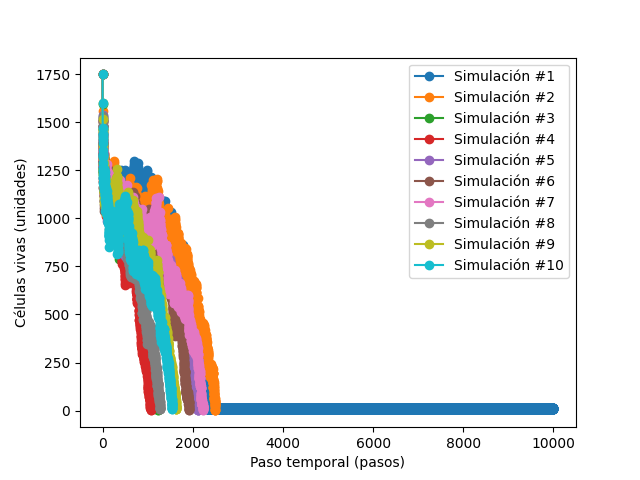
\includegraphics[width=0.8\linewidth]{collapse3d/size_i30}
    \caption{Cantidad de celdas vivas en el tiempo del sistema de Colapso Cúbico con $initialLiveCellsProportion = 0.3$}
    \label{fig:colapso3d_i30}
\end{figure}
\begin{figure}[H]
    \centering
    \includegraphics[width=0.8\linewidth]{collapse3d/size_i90}
    \caption{Cantidad de celdas vivas en el tiempo del sistema de Colapso Cúbico con $initialLiveCellsProportion = 0.9$}
    \label{fig:colapso3d_i90}
\end{figure}

Como se puede apreciar en la fig. \ref{fig:colapso3d_i30}, el sistema alcanza el equilibrio
antes del paso temporal 4000, por lo que se hace el análisis del observable en el paso temporal mencionado.
Analizando las figs. \ref{fig:colapso3d_i10} y \ref{fig:colapso3d_i90}, se
puede notar las tres órdenes de magnitud de diferencia en la cantidad de pasos temporales necesarios para
alcanzar el equilibrio.
Es por ello que se decidió estudiar la cantidad de celdas vivas en el equilibrio y su pendiente de crecimiento,
en función de la densidad de celdas vivas en el dominio inicial.

\begin{figure}[H]
    \centering
    \includegraphics[width=0.8\linewidth]{collapse3d/size_vs_input}
    \caption{Cantidad de celdas vivas en función del input para el sistema de Colapso Cúbico}
    \label{fig:colapso3d_size_vs_input}
\end{figure}
\begin{figure}[H]
    \centering
    \includegraphics[width=0.8\linewidth]{collapse3d/size_slope_vs_input}
    \caption{Pendiente de crecimiento de cantidad de celdas vivas en función del input para el sistema de Colapso Cúbico}
    \label{fig:colapso3d_size_slope_vs_input}
\end{figure}

Se puede comprar en la fig. \ref{fig:colapso3d_size_vs_input} que la cantidad de celdas vivas en el equilibrio
resulta diezmada para cualquier valor de $initialLiveCellsProportion$, alcanzando un valor máximo de aproximadamente
60 celdas vivas, lo cual resulta casi nulo para una matriz de $50 \times 50 \times 50$ ya que representa una densidad
de $60/(50 \times 50 \times 50) \times 100 = 0.048\%$.
Por otra parte, se puede observar en la fig. \ref{fig:colapso3d_size_slope_vs_input} que la pendiente de
crecimiento es negativa para cualquier valor de $initialLiveCellsProportion$, y su módulo aumenta
considerablemente a medida que crece la densidad inicial de celdas vivas.
Aunque la cantidad de celdas vivas en el equilibrio disminuye con respecto al paso inicial, no se puede afirmar
que dichas celdas vivas se encuentren en el centro del dominio inicial, ya que pueden estar distribuidas de manera
aleatoria en la totalidad de la matriz.
Por lo tanto, se ha decidido estudiar la distancia de la celda viva más lejana al centro del dominio en función del
paso temporal.

\begin{figure}[H]
    \centering
    \includegraphics[width=0.8\linewidth]{collapse3d/distance_i10}
    \caption{Distancia de la celda viva más lejana al centro en función del tiempo con $initialLiveCellsProportion = 0.1$}
    \label{fig:colapso3d_d10}
\end{figure}
\begin{figure}[H]
    \centering
    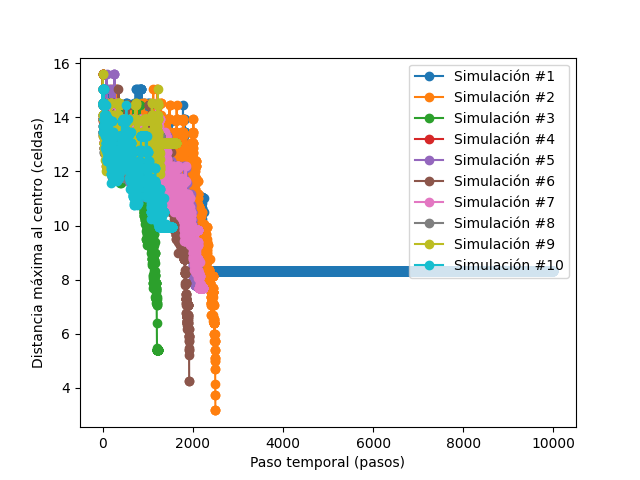
\includegraphics[width=0.8\linewidth]{collapse3d/distance_i30}
    \caption{Distancia de la celda viva más lejana al centro en función del tiempo con $initialLiveCellsProportion = 0.3$}
    \label{fig:colapso3d_d30}
\end{figure}
\begin{figure}[H]
    \centering
    \includegraphics[width=0.8\linewidth]{collapse3d/distance_i90}
    \caption{Distancia de la celda viva más lejana al centro en función del tiempo con $initialLiveCellsProportion = 0.9$}
    \label{fig:colapso3d_d90}
\end{figure}

